%
\section{Results and Remarks}
%
Because its description is based on Lemma~1, which does not provide an equivalency condition
for finding $\theta_1^*, \theta_2^*, \ldots, \theta_N^*$, the performance of Algorithm~1 will
in general not achieve the optimum result for SNR Boost \cite{b1}.

\begin{figure}[!t]
\centering
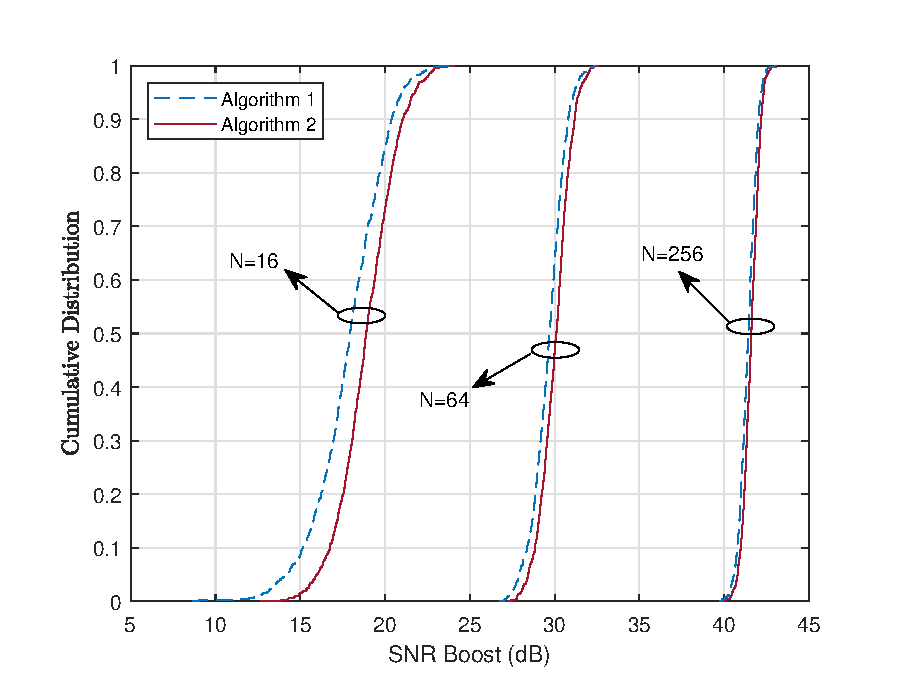
\includegraphics[width=0.45\textwidth]{Overall_K2_N_16_64_256.eps}
%\includegraphics[width=0.5in]{3d_figures/TW_CT_combined_original_QLOS.eps}
%\includegraphics[width=0.5in]{3d_figures/TW_CT_combined_original_QNLOS.eps} \\
\caption{CDF plots for SNR Boost with Algorithm 1 and Algorithm 2, $K=2$.}
 \label{fig:SNRBoostK2}
 \end{figure}
\begin{comment}
 \begin{figure}[!t]
\centering
\includegraphics[width=0.45\textwidth]{Overall_K4_N_16_64_256.eps}
%\includegraphics[width=0.5in]{3d_figures/TW_CT_combined_original_QLOS.eps}
%\includegraphics[width=0.5in]{3d_figures/TW_CT_combined_original_QNLOS.eps} \\
\caption{CDF plots for SNR Boost with Algorithm 1 and Algorithm 2, $K=4$.}
 \label{fig:SNRBoostK4}
 \end{figure}
\end{comment}
We have implemented Algorithm~1 to the best of our interpretation. We have also implemented
Algorithm~2.
We present the CDF results for SNR Boost \cite{b1} in Fig.~\ref{fig:SNRBoostK2} for $K=2$
and $N =16$, $64$, and $256$, using the average of 1,000 realizations of the channel.
Clearly,
Algorithm~1 is not optimal. Algorithm~2 performs better than Algorithm~2 although the
gains decrease with $N$. Plots for $K=4$ show smaller gains as compared to $K=2$, but
still, Algorithm~2 always performs better than Algorithm~1 for the same $K$ and $N$.

We note that it is possible to convert the maximization of $\cos(\theta_n+\alpha_n-\phase{\mu})$
to the minimization of a simple expression. For example, minimization of $f_1(x)=
\pi - | (x \!\! \mod 2\pi ) - \pi |$ is the same as maximization of $\cos(x)$ within
the context of Lemma~2. However, this is different than minimization of $|x \!\! \mod 2\pi|$
proposed in Lemma~1 of \cite{b1}. The reason can be
seen by plotting these functions against $x$. While $f_1(x)$ and $\cos(x)$, in
addition to being periodic with period $2\pi$, have even symmetry around odd
multiples of $\pi$, $| x \!\! \mod 2\pi |$ (or equivalently, $(x \!\! \mod 2\pi)$) does not
have this symmetry.

